% Uncomment one of three below
%\RequirePackage[]{optional}
\RequirePackage[notslides]{optional}
%\RequirePackage[slides]{optional}

\opt{slides}{
% Following for presentation mode
\documentclass[10pt]{beamer}
\usepackage{xmpmulti}
%usetheme{Berlin}
}
\opt{notslides}{
% Following for notes mode
\documentclass[a4paper]{article}
\usepackage{beamerarticle}
\usepackage{a4wide}
\usepackage{graphicx}
\usepackage{amsfonts}
\usepackage{fancyhdr}
}

% Following for all modes
%\usepackage{auto-pst-pdf}
%\usepackage{pst-pdf}
\usepackage{psfrag}

\parindent=0ex
\parskip=1ex
\newcommand{\conv}{\ast}
\reversemarginpar

%\title{Introduction:  applications of signal theory}
%\author{}
%\date{}

\begin{document}
\pagestyle{fancy}
\fancyhead{}
\renewcommand{\headrulewidth}{0pt}
\fancyfoot[C]{\thesection-\thepage}

\begin{frame}
  \titlepage
\end{frame}

\section{Introduction:  applications of signal theory}

%\mode<article>{{\bf \LARGE Introduction:  applications of signal theory} \newline}

\subsection{Mechatronics example}

In chemical engineering one often has to deal with streams of liquid.  Suppose one wants to measure the concentration of a known substance in water.  It could be something desirable, like a valuable hydroxytyrosol molecule, or something undesirable, like leftover tannins after an extraction process.  We simplify the problem by assuming that there is only one type of substance present in the stream, but its concentration is unknown.

One solution is to use the optical transmission properties of liquids to make an optical sensor for the concentration measurement.  Using a transparent pipe (or a flow cell) we shine a light from one side, through the liquid stream, and measure the intensity on the other side.
\begin{center}
  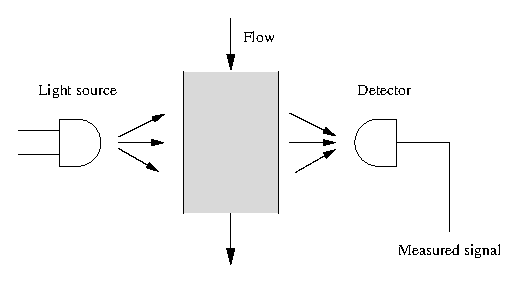
\includegraphics{beerlambertcell}
\end{center}
If there is pure water in the pipe there will be no absorption, and the light intensity at the output will be high; if there is a high concentration of black goo in the pipe then the light will almost all get absorbed while traveling through the liquid, and the light intensity at the output will be low.  We can measure the light intensity at the output using a photodiode, which with a bit of electronics can turn light intensity into volts.
% http://en.wikipedia.org/wiki/File:Dilution-concentration_simple_example.jpg released to public domain
\begin{center}
  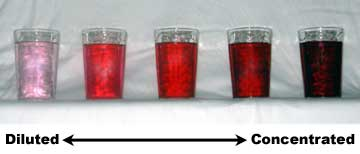
\includegraphics{Dilution-concentration_simple_example}
\end{center}

The Beer-Lambert law characterises the absorption or transmission properties of a substance:
\begin{equation*}
  I = I_0 e^{-\epsilon l c}.
\end{equation*}
Here $\epsilon$ is the absorption coefficient of the substance being measured, and is assumed known.  The optical path length through which the measurement is being taken is $l$, which we also assume known.  The quantity $c$ (in say grams/liter) is the thing we're trying to find.  The light intensity at the output is $I$, and we measure this.  Evidently then $I_0$ is the output intensity when the concentration $c$ is zero, in other words when the liquid stream is pure water --- we can find this value simply by measuring the output light intensity through pure water in a calibration stage.  Now, for a stream that isn't pure water, we can find the concentration by measuring the output light intensity $I$, and solving for $c$ (since all other quantities are known).

The procedure just described assumes that the light is on all the time (or at least all the time while any measurements are being taken).  There's a problem, though --- what if there's another source of light that contributes to the signal at the photodiode?  For example, if the system is outdoors then sunlight will also contribute to the received signal and this contribution may vary with time (say as clouds move past).  In this case, if we sample the light intensity through time we will see the superposition of two components (with noise, which is always there):
\begin{center}
  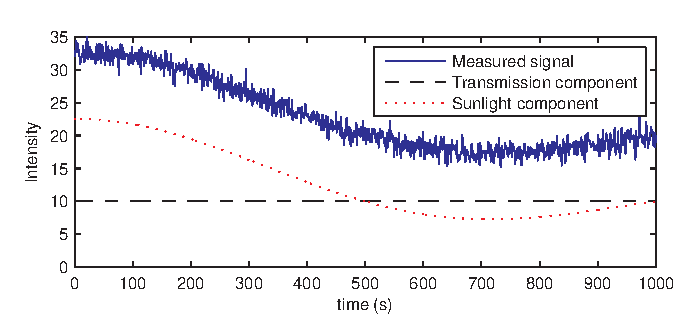
\includegraphics{me_example1}
\end{center}
Now measuring the intensity tells us very little about the concentration.

The most obvious way of fixing this problem is to put everything into a lightproof box which no sunlight can enter.  While this is the best engineering solution we're assuming that it's not possible for some reason.

We can resolve the problem if we can control of the light source.  If the light is on, then we measure the combined contribution from the transmitted signal and the sunlight;  if the light is off then we measure the sunlight component alone.  The difference between these two signals is just the transmitted component, and we can find the concentration of the liquid.  Thus by taking a {\em differential} measurement we have eliminated the {\em common mode} signal --- in this case the sunlight.

We can't take the two measurements simultaneously, since we only have one photodiode, so the best thing to do is to pulse the light on and off quickly, taking measurements with light on and light off, and subtract successive samples.  If the contribution of the signal caused by sunlight varies quite slowly then the fact that the two measurements are actually separated in time is insignificant.  This process is called {\em coherent detection}.

Turning the light source on and off means that we are effectively varying $I_0$ in the Beer-Lambert equation as a function of time.  If the concentration $c$ is (roughly) constant then we can explicitly  write the time-varying relationship as
\begin{equation*}
  I(t) = I_m(t) e^{-\epsilon l c}.
\end{equation*}
In the pulsed situation just described the signal $I_m(t)$ is a square wave, switching between zero and the value $I_0$.  In general though, since we have control of the source, we could use {\em any} excitation signal for this purpose.  In particular, we could choose a sinusoid of frequency $w_c$, suitably offset so that it also ranges between zero and $I_0$:
\begin{equation*}
  I_m(t) = \frac{I_0}{2} ( \sin(\omega_c t) + 1 ) = \frac{I_0}{2} \sin(\omega_c t) + \frac{I_0}{2}.
\end{equation*}
Ignoring the offset term we see that we are effectively multiplying the light source intensity by a sinusoid of frequency $\omega_c$.
This process is called {\em modulation}, and we can say that we are modulating the light source with a frequency $\omega_c$.

The light intensity at the output after transmission through the sample is now
\begin{equation*}
  I(t) = \frac{I_0}{2} e^{-\epsilon l c} \sin(\omega_c t) + \frac{I_0}{2} e^{-\epsilon l c},
\end{equation*}
which has a sinusoidal component of amplitude $\frac{I_0}{2} e^{-\epsilon l c}$ oscillating at frequency $\omega_c$, and an additional non-oscillating component.  Note now that the peak-to-peak magnitude of the sinusoidal component is $I_0 e^{-\epsilon l c}$, and if we can measure this then we can estimate the actual value for the concentration $c$.

When the effect of sunlight and noise is included the components of the signal at the photodiode receiver are as follows:
\begin{center}
  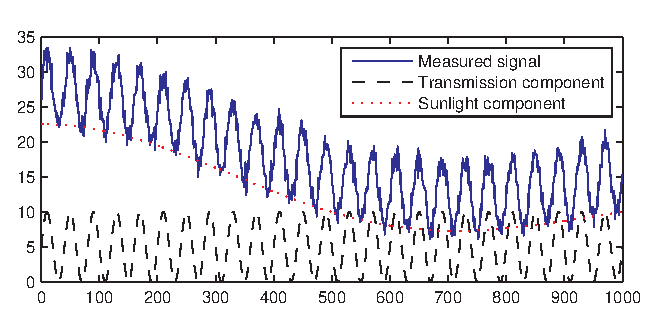
\includegraphics{me_example2}
\end{center}
\vspace*{0.2ex}
The problem now is to use the measured signal to make an estimate of concentration.  Unlike in the previous case, though, this can apparently be done:  as long as the interfering sunlight component varies much more slowly than the sinusoidal modulation then we have a sense that we should be able to separate the slowly-varying components (sunlight and offset) from the sinusoidal component at frequency $\omega_c$.  This can be done by putting the signal through a system that removes low frequency components, and only passes high input frequencies to the output --- a highpass filter.

\subsection{Power engineering example}

Electrical power systems and distribution networks are often based on 3-phase alternating current.  
% http://en.wikipedia.org/wiki/File:Three_Phase_Electric_Power_Transmission.jpg
\begin{center}
  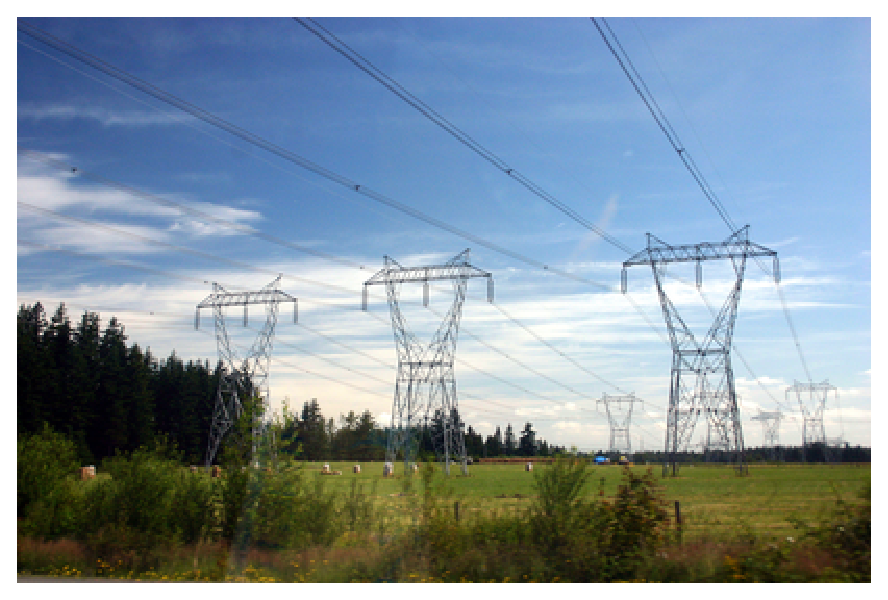
\includegraphics[width=9cm]{threephasepower}
\end{center}
A 3-phase system consists of three conductors carry alternating currents, each at the same frequency but with a phase difference of 120 degrees between them.    If the phases are balanced and the phase currents are perfect 50 Hz sinusoids then they cancel one another out, and no common neutral wire is required.  In practice, to accommodate unbalanced loads a neutral conductor may be  present, but with a reduced size.  This means that less conductor material is required to transmit electrical power than equivalent single-phase or two-phase systems at the same voltage, so costs are lower.  (The construction of a high voltage transmission line costs in the vicinity of R1 million per kilometer.)  There are also other reasons to use 3-phase power.

In a 50 Hz 3-phase power system, the currents in each of the phases need to be 50Hz sinusoids with relative phases of 120 degrees for the current in the neutral conductor to be exactly zero.  However, when nonlinear loads are attached to a power system it generates harmonics at integer multiples of the fundamental frequency (in this case at frequencies 100Hz, 150Hz, etc.).  These harmonics increase the current in the neutral  conductor, and cause power quality problems that can cause the system to fail.  Basically, harmonic frequencies in a power grid are very undesirable.

{\em Suppose\marginpar{\bf Exercise:} the currents in three phases of a 50Hz power system are $i_1(t) = \sin(2 \pi (50) t)$, $i_2(t) = \sin(2 \pi (50) t + 2 \pi/3)$, and $i_3(t) = \sin(2 \pi (50) t + 4\pi/3)$.  These phases are all separated from one another by a phase difference of $2 \pi/3$ radians or $120$ degrees.  Show that the total sum of the currents in these phases is zero for all time.  It may be useful to use the identity $\sin(x) = \frac{1}{2} (e^{j x} - e^{-j x})$.}

Suppose we want to transmit power between two distant points.  Power lines are not ideal conductors:  they have resistance and stray capacitance and inductance, so what you put in the one side is not necessarily what you get out of the other.  In signals and systems theory it is common to develop an abstract mathematical model of the system (in this case the transmission line) in terms of an input-output relationship.  This is a mathematical model that allows you to calculate the output signal from the system for any given input signal.  In practice this model is often obtained from physical principles, where the input-output relationship can be expressed in terms of a differential equation.  A differential equation relating the input of a transmission line to its output can be derived in this way (and you may see the formulation in later courses).

Some systems have nice properties.  Suppose $x(t)$ is the input to a system, $y(t)$ the output, and the input-output relationship is given by $y(t) = 10 x(t - 5)$.  This system takes a signal $x(t)$, delays it by 5 time units, and multiplies the result by 10.  If the input is a sinusoidal signal $x(t) = \sin(\omega_c t)$, then the output is $y(t) = 10 \sin(\omega_c (t-5)) = 10 \sin(\omega_c t - 5 \omega_c)$.  This output is a sinusoid, oscillating {\em at the same frequency} $\omega_c$ as the input.  The system therefore doesn't generate any frequencies that were not already in the input signal.  Alternatively, a system like this doesn't generate any harmonics of the input:  if the input signal is a sinusoid at 50Hz, then the output signal only contains alternating components at 50Hz.  A system like this is very friendly to power networks.

Consider now a system with the input-output relationship $y(t) = \{x(t)\}^2$.  At any instant in time this system produces a signal at the output that is the square of the value of the signal at the input at the same time instant.  The same sinusoidal input as before now produces the output 
\begin{equation*}
  y(t) = \{ \sin(\omega_c t) \}^2 = \sin^2(\omega_c t) = \frac{1}{2} (1 - \cos(2 \omega_c t)) = \frac{1}{2} - \frac{1}{2} \cos(2 \omega_c t)).
\end{equation*}
The output therefore consists of two components:  a constant component and an oscillating component at frequency $2 \omega_c$.  Thus, while the input only contained a single frequency at 50Hz, the output contains a component at frequency 100Hz:  the system has generated a first harmonic, which is a sign of trouble in power networks.

Finally, consider the system with the input-output relationship $y(t) = \{x(t) + 1\}^2$, which adds one to the input and then squares the result.  For the input $x(t) = \sin(\omega_c t)$ the input and output are shown below:
\begin{center}
  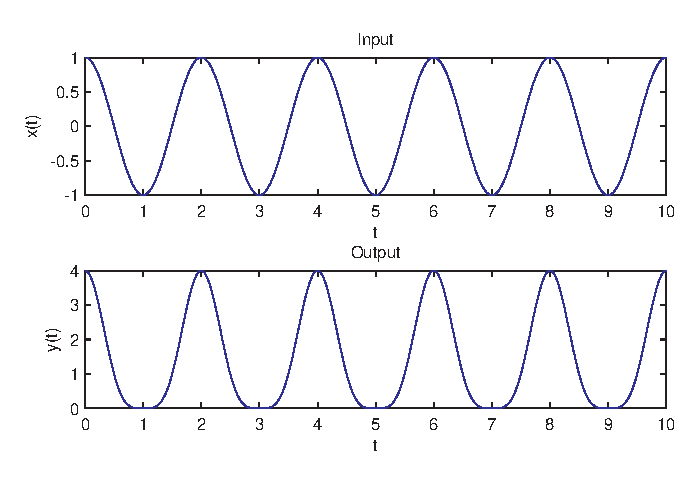
\includegraphics{ee_example}
\end{center}
The output is no longer even sinusoidal:  it is the superposition of a set of sinusoidal components each with different amplitudes.  The ideas of signals and system analysis allows one to determine the harmonics that are present in this signal, and quantify their magnitudes.  This represents a lot of useful information to a power engineer that worries about these things.

The systems that have nice properties with respect to generating harmonics of an input frequency at the output are called {\em linear} systems.

\subsection{Telecommunications example}

Suppose you want speak to somebody very far away.  When a person talks, it causes an acoustic pressure wave which propagates through the atmosphere.  This wave corresponds to physical movement of air molecules and, while the molecules themselves don't each move very far, the pattern (or wave) of movement propagates and the speech signal is contained (or encoded) in this changing pressure pattern.  When the pressure wave impinges on the tympanic membrane of a listener, the signal is decoded by the ear (and the brain) and the message is received.

Since gasses generally resist motion and it takes energy to physically move air molecules, acoustic pressure waves decay quite rapidly as you move away from the source.  The distance between the speaker and the listener is therefore quite restricted with this mode of communication.  Electromagnetic radiation, on the other hand, at least through a vacuum propagates without energy loss (which is why we can see light from at the edge of the universe that has travelled about 12 billion light years without apparent decay).  So if we can encode a speech signal onto a radio wave, and decode it on the other side, we can communicate over huge distances.

Microphones turn acoustic speech signals into electrical signals, and speakers turn electrical signals into acoustic signals.  In turn, antennas can convert both ways between electrical signals and electromagnetic radiation.  A seemingly reasonable approach could therefore be to do the following:
\begin{center}
  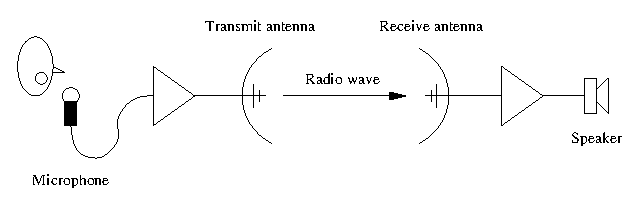
\includegraphics{radiocomms1}
\end{center}
The triangular blocks are amplifiers that boost the signals (by multiplying them by a value greater than 1).

There are two problems, though, related to the frequencies present in speech.  The human throat is also a vibrating structure that produces acoustic pressure waves in the air, and we can't really produce sounds at frequencies greater than around 5kHz.  The signal coming in from the microphone and going out to the antenna will thus produce EM radiation at frequencies up to about 5kHz.  The first problem is that the atmosphere happens to absorb radiation at this frequency quite strongly, so the signal wont propagate very far.  The second is a bit more complicated, and deals with the way that antennas interact with electromagnetic radiation:  the size of the antenna relates to the wavelength of the radiation that it is being transmitted or received.  Since $v = f \lambda$ and $v$ for light is $c$, a frequency of 5kHz for EM radiation has $\lambda = 3 \times 10^8/5000 = 60000$m.  We therefore need an antenna at least about 60km big to do the job, which is practically ridiculous.

The solution is to modulate:
\begin{center}
  \psfrag{s(t)}{\scriptsize $s(t)$}
  \psfrag{cos(wct)}{\scriptsize $\cos(\omega_c t)$}
  \psfrag{s(t)cos(wct)}{\scriptsize $s(t) \cos(\omega_c t)$}
  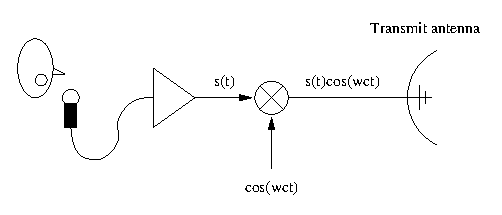
\includegraphics{radiocomms2}
\end{center}
The speech signal from the microphone is $s(t)$ is multiplied by a sinusoidal signal at a selected carrier frequency $\omega_c$, so the signal going into the antenna is now $x(t) = s(t) \cos(\omega_c t)$.  It's quite simple to do this multiplication in electronics, and nowadays you can buy little integrated circuits (8 pin chips) that do it.  The signals $s(t)$ and $x(t)$ are shown in the first two plots below:
\begin{center}
  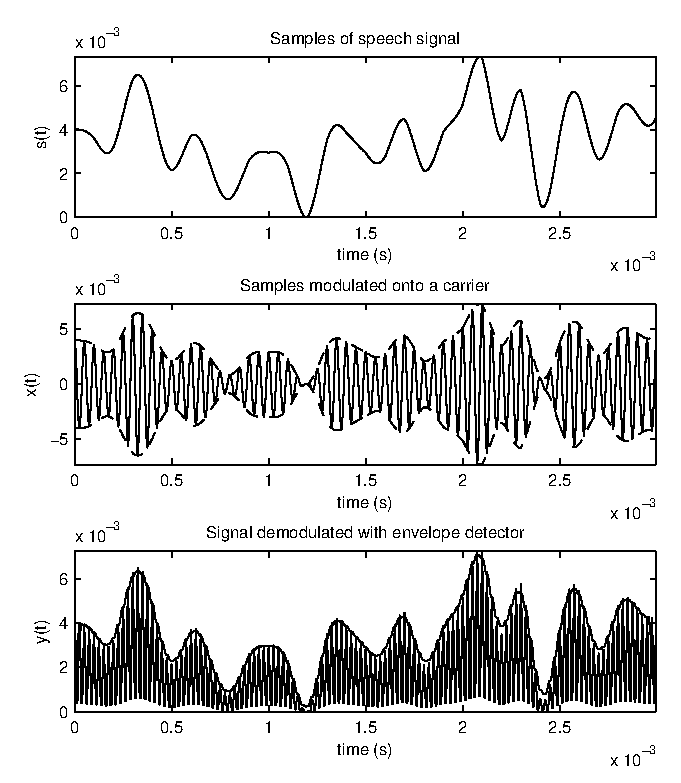
\includegraphics{ec_example}
\end{center}
The signal $s(t)$ is now {\em modulated} onto the amplitude of the carrier wave, and this mechanism is called amplitude modulation (or AM).  The "size" of the sinusoid at any time is the required signal.  The important thing is that the signal $x(t)$ now effectively oscillates at the frequency of the carrier, which can be as high as we want.

Say we choose a carrier frequency of 100MHz.  The wavelength of the EM radiation emitted by the antenna is then $\lambda = 3 \times 10^8/100 \times 10^6 = 3$m.  You can make a pretty lousy antenna with a size (or length) that is about a quarter of a wavelength, or in this case $0.75$m.  That's quite reasonable:  it's about as big as the aerial of an FM radio receiver, which usually tunes into frequencies from about 87MHz to 108MHz.  Alternatively, think about cell phones.  One of the GSM frequency bands often allocated to them is 1800MHz, for which a wavelength is about 16cm.  A quarter wave antenna is then around 4cm, which is handy for a pocket mobile device.  

Radiation at frequencies such as those mentioned above propagate quite easily through the atmosphere, so we can essentially send the signal $x(t)$ wherever we want it.  (Different frequencies do have different propagation properties, though.)  We can receive it using roughly (or exactly) the same antenna we used to transmit it, so any listener can in principle see the signal $x(t)$.  

Recovering $s(t)$ from $x(t)$ in the case of amplitude modulation can be done quite simply.  If you put $x(t)$ through a system that squares its value at each point in time, the output is the very rapidly varying signal $y(t)$ at the bottom of the previous figure.  The "height" of the sinusoid at any instant carries the signal $x(t)$.  Building electronics to ignore the fast variations and track this height is quite easy, so the signal $s(t)$ can be recovered.

Quite strangely, another way to recover the signal is to multiply $x(t)$ with $\cos(\omega_c t)$ again.  The result of this operation is
\begin{equation*}
  z(t) = x(t) \cos(\omega_c t) = s(t) \cos^2(\omega_c t) = s(t) \left( \frac{1}{2} + \frac{1}{2} \cos(2 \omega_c t) \right)
  = \frac{1}{2} s(t) + \frac{1}{2} s(t) \cos(2 \omega_c t).
\end{equation*}
The component $\frac{1}{2} s(t)$ oscillates at a frequency of about 5kHz, since that's the highest frequency in $s(t)$.  The component $\frac{1}{2} s(t) \cos(2 \omega_c t)$ oscillates at a frequency of about $2 \omega_c$, which is usually {\em much} higher than 5kHz.  We can therefore recover $s(t)$ (or acutally $\frac{1}{2} s(t)$) by putting $z(t)$ though a system that filters out high frequencies --- a low pass filter.  After the signal is recovered it can be amplified as required, and played back through a speaker to create a modulated pressure wave which a human listener can again receive and decode.  

\end{document}
